\section{Kalman Filter}

According to the professor, when we talk about autonomous driving the most important tool is the \textbf{Kalman filter}.

\subsection{Motivation}
So far, in perception, we have identified the objects in each frame (for example with clustering).
This approach has two problems: we do not know \textbf{how} the objects are moving, and if we only use the obstacles detected at each iteration, we never see the \textbf{present}, but always the past.

\begin{figure}[H]
    \centering
    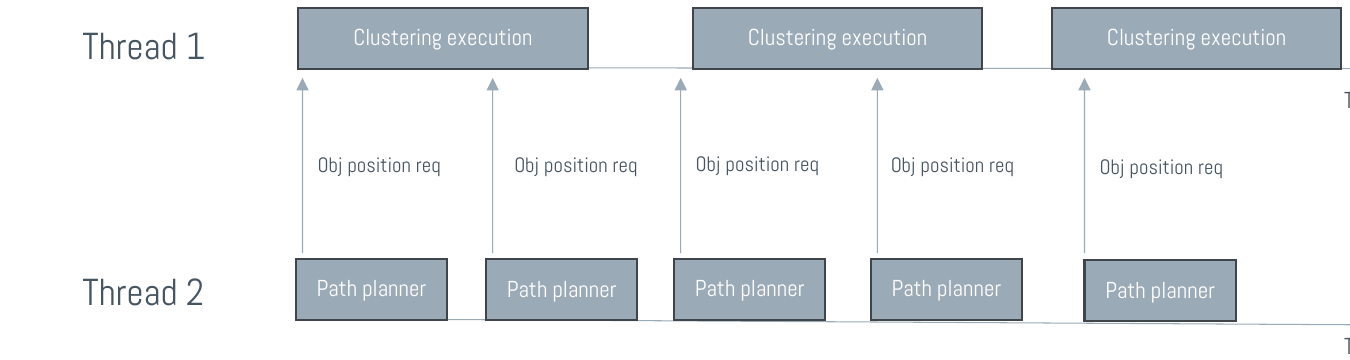
\includegraphics[width=0.75\textwidth]{images/C5_1.png}
    \caption{Clustering and path planner running on two different threads}
\end{figure}

An AD stack is a \textbf{multi-threaded} and \textbf{asynchronous} system.
For example, the path planner periodically asks the perception which obstacles are in the world and where they are, but the two tasks run on different threads and are not temporally aligned: when the request arrives, the perception may not have the object position for that exact instant, so the path planner ends up working on \textbf{old perception}.
It is therefore very useful to \textbf{predict} where the object should be \textbf{now}.
\begin{figure}[H]
    \centering
    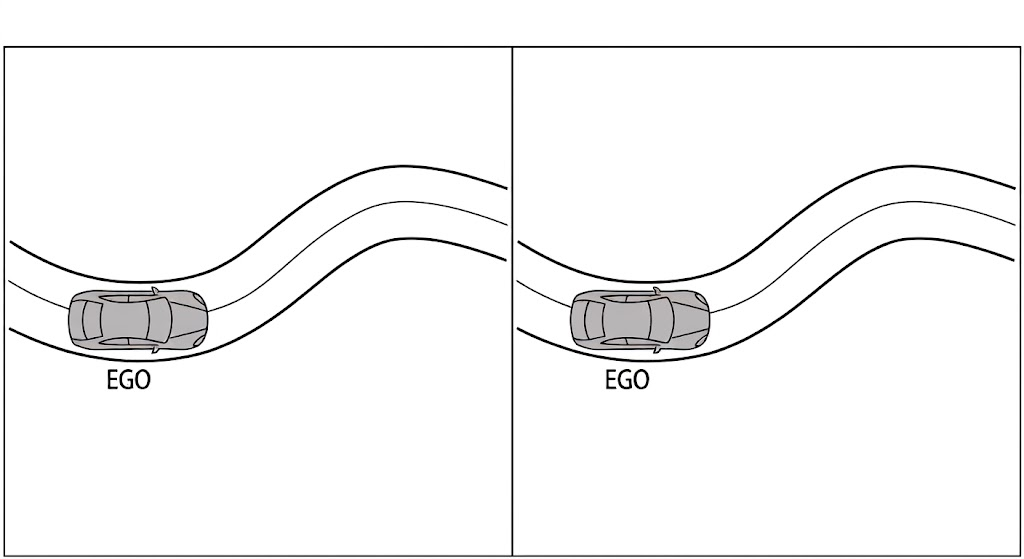
\includegraphics[width=0.35\textwidth]{images/C5_2.png}
    \caption{What the software sees vs reality}
\end{figure}

The Kalman filter allows us to \textbf{estimate the state of an object over time}.
We are not just interested in the movement in the scene, but in \textbf{who} is moving and \textbf{how}.
The filter does two things:
\begin{compactitemize}
    \item \textbf{Prediction}: predict the current/future state, to compensate for the temporal latency;
    \item \textbf{Update}: filter the measurement noise and fuse the data coming from uncertain sensors.
\end{compactitemize}

\subsection{An intuitive example}
Let's suppose that we are tracking our own position in a \textbf{1D world}, walking in a room at \textbf{1\,m/s}.
With our eyes open, it is very easy to know where we will be after 4 seconds: using basic kinematics, $p' = p + v\Delta t$.
So, based on our \textbf{kinematics} (and on our eyes, i.e.\ our \textbf{sensors}), we can estimate our position.

Now we \textbf{close our eyes} (and we do not even know exactly where we started) and keep walking for 4 seconds.
We can still estimate our position with the kinematics, but this is only an \textbf{estimated guess}: a guess is not perfect, and the longer we walk, the more our estimate deteriorates, so the \textbf{certainty} about where we are decreases over time.
In the Kalman world this step is called \textbf{prediction}.

At some point we \textbf{open our eyes}, i.e.\ we acquire new information from the sensors.
We compare the prediction with the visual measurement and \textbf{combine them in a weighted manner}, weighting how much we trust the eyes and the kinematic model.
In this way we update both the estimate of where we are and our certainty about it.
In the Kalman world this step is called \textbf{update} (or \textbf{correction}).

But what happens if our kinematic model is wrong, or if the floor slips? This is the error coming from the \textbf{external world} (the model of the motion is not perfect).
And what if we are wearing the \textbf{wrong glasses}? Then we barely know where we are, and the weight of the visual information must decrease.
We still improve our estimate with respect to walking with closed eyes, but we must take into account that \textbf{sensors are not perfect} either (think about GPS or LiDAR): this is the \textbf{sensor noise}.
The Kalman filter introduces variables that model exactly these two errors: how wrong our motion model is, and how wrong our sensors are.

\subsubsection{Bayesian inference}
What we have just done is \textbf{Bayesian inference}: a statistical method that \textbf{updates our belief} in a hypothesis as new evidence becomes available.
Its mathematical framework is the \textbf{Bayes theorem}:
\[
P(x_k \mid z_k) = \frac{P(z_k \mid x_k)\, P(x_k)}{P(z_k)}
\]
where:
\begin{compactitemize}
    \item the \textbf{prior} $P(x_k)$ is the kinematic prediction, what we expect before seeing the sensor data (``I drove at 50\,km/h for 10 seconds, so I should be at 500\,m'');
    \item the \textbf{likelihood} $P(z_k \mid x_k)$ is the sensor observation, the probability of measuring $z_k$ if the true state were $x_k$ (``if I really were at $x_k$, how likely is it that the GPS reads $z_k$?'');
    \item the \textbf{posterior} $P(x_k \mid z_k)$ is the fusion: multiplying prior and likelihood we obtain a narrower Gaussian (lower variance), and the optimal estimate is placed where both sources agree. For example, if the wheels say 100\,m and the GPS says 103\,m, the car trusts neither of them blindly and places the estimate at 102\,m.
\end{compactitemize}

\begin{infobox}[The brain as a Bayesian prediction machine]
Many cognitive scientists and philosophers (e.g.\ Andy Clark, Karl Friston) see the brain as a ``Bayesian prediction machine'', which constantly updates its prior beliefs using the senses.
Friston formalized this idea in the \textbf{free energy principle}: living beings act and update their internal model of the world in order to \textbf{minimize surprise}, i.e.\ the difference between what they predict and what they perceive.
\end{infobox}

\subsection{The Kalman filter}
\begin{wrapfigure}{R}{0.41\textwidth}
    \centering
    \vspace{-10pt}
    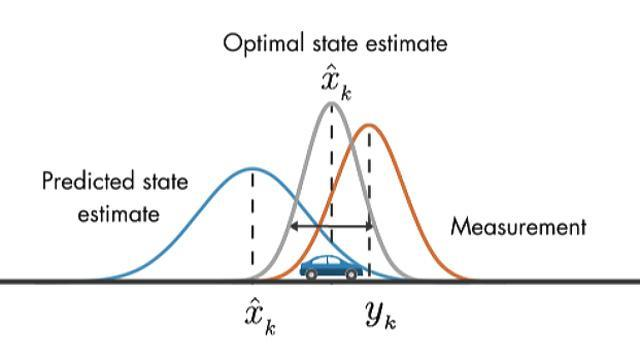
\includegraphics[width=0.4\textwidth]{images/C5_3.png}
    \caption{The estimate combines prediction and measurement}
    \vspace{-10pt}
\end{wrapfigure}
The \textbf{Kalman filter} is an analytical implementation of the Bayes theorem: it applies this \textbf{recursive Bayesian inference} at each time step to continuously estimate the true state of a system from noisy measurements.
It was created in 1960 by Rudolf E.\ Kalman and was used for the trajectory estimation of the Apollo program.

In other words, it is a technique for \textbf{estimating the state of a system}: a mathematical process that uses equations and data (e.g.\ from the sensors) to estimate a value of the objects, such as their position or velocity.
It is used both to \textbf{correct} the values (since sensors are not perfect) and to \textbf{predict} them.

\begin{infobox}[Kalman filter and Apollo XI]
\begin{minipage}[c]{0.6\linewidth}
On the Apollo missions the Kalman filter ran on the Apollo Guidance Computer (AGC) for real-time navigation.
It combined the measurements of the inertial sensors with radio/optical updates to estimate the spacecraft position, velocity and attitude, together with the uncertainty covariance $P$.
The estimate was then used by the AGC to control engine burns and the re-entry trajectory.
\end{minipage}\hfill
\begin{minipage}[c]{0.36\linewidth}
    \centering
    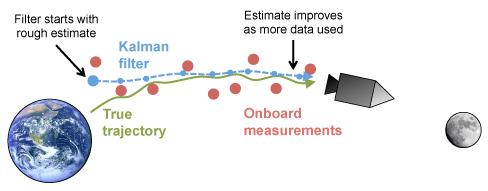
\includegraphics[width=\linewidth]{images/C5_4.png}
\end{minipage}

\vspace{6pt}
\centering\small
\begin{tabular}{|l|p{6.5cm}|l|}
    \hline
    \textbf{Source} & \textbf{Description} & \textbf{Frequency} \\
    \hline
    IMU & Accelerometers and gyros: specific force and angular rates & Continuous ($\sim$10\,Hz) \\
    \hline
    Sextant / optical tracker & Angles between stars and landmarks (Earth, Moon) & Manual / periodic \\
    \hline
    Remote station updates & Astronaut or ground-based corrections & As needed \\
    \hline
    Process model ($F$, $B$, $u$) & Physics-based propagation with Newton's equations & Continuous \\
    \hline
\end{tabular}
\end{infobox}

\subsubsection{How it works}
The goal of the Kalman filter is to obtain a \textbf{probabilistic estimate of the state} of the vehicle and to update it in real time, cycling between two steps after an initialization:
\begin{compactitemize}
    \item \textbf{Prediction}: uses the \textbf{kinematic (motion) model}, which defines how the vehicle evolves over time (IMU, car information, \dots);
    \item \textbf{Correction} (or \textbf{update}): uses the information of GPS/radar/LiDAR to correct the previous prediction through the \textbf{measurement model}. New measurements give us information with a small variance.
\end{compactitemize}

\begin{figure}[H]
    \centering
    \begin{subfigure}{0.35\textwidth}
        \centering
        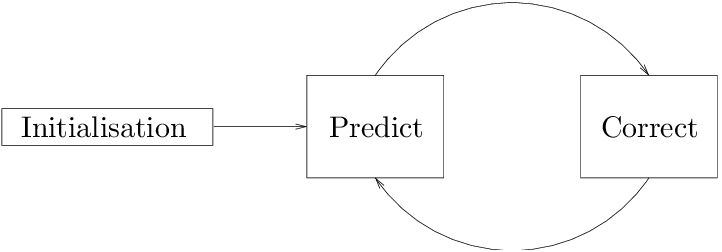
\includegraphics[width=\linewidth]{images/C5_5.png}
        \caption{The Kalman filter cycle}
    \end{subfigure}\hfill
    \begin{subfigure}{0.6\textwidth}
        \centering
        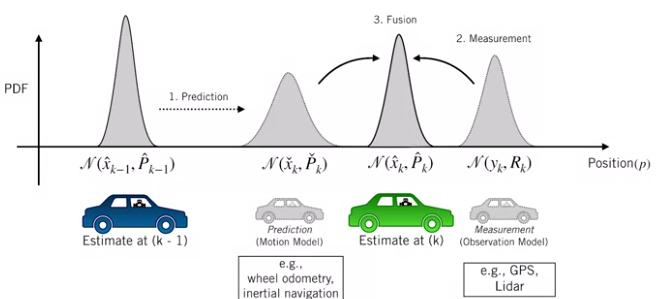
\includegraphics[width=\linewidth]{images/C5_6.png}
        \caption{Prediction, measurement and fusion}
    \end{subfigure}
    \caption{Prediction and correction steps}
\end{figure}

For example, consider a vehicle with a navigation system based on GPS and vehicle information.
We start by reading the sensor to \textbf{initialize} the position tracker.
Then we use the dynamics of the vehicle to \textbf{predict} how it moves, for instance with a constant velocity model: $location = previous\ location + velocity \cdot \delta t$, where $\delta t$ is the time elapsed between two measurements.
This prediction is uncertain, so we represent it as a probability distribution (a \textbf{Gaussian}) describing where the vehicle is likely to be.

When a new GPS reading arrives, the sensor provides an observed position (\textbf{update}).
This measurement is also uncertain, so it has its own distribution.
The Kalman filter merges the two distributions, the predicted state (from the motion model) and the measured one (from the sensor), and obtains a new and more accurate estimate of the position and of its uncertainty (\textbf{correction}).
Mathematically, this is achieved by \textbf{minimizing the estimation error covariance}, which means giving more weight to the more reliable source.

\subsubsection{Implementation types}
Prediction and correction do not necessarily run at the same frequency, and there are two possible implementations.

\noindent\begin{minipage}[c]{0.55\textwidth}
In the \textbf{sequential} implementation, every measurement arrives at the same rate as the prediction step, so each prediction is followed by a correction.
Typical use cases are a single sensor, hardware-synchronized sensors, or the offline processing of logged data.
\end{minipage}\hfill
\begin{minipage}[c]{0.41\textwidth}
    \centering
    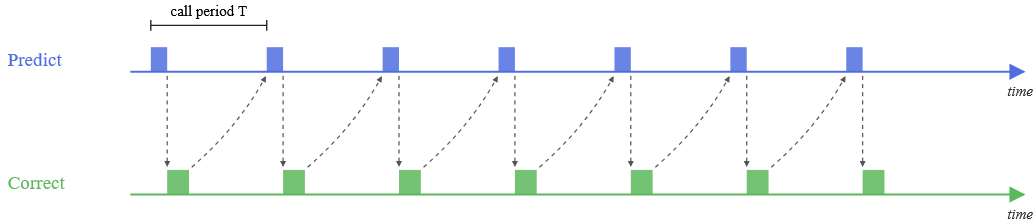
\includegraphics[width=\linewidth]{images/C5_7.png}
    \captionof{figure}{Sequential: one correction per prediction}
\end{minipage}

\begin{table}[H]
    \centering
    \begin{tabular}{|p{7.5cm}|p{7.5cm}|}
        \hline
        \textbf{Pros} & \textbf{Cons} \\
        \hline
        Simple to implement and debug & Needs synchronized measurements \\
        \hline
        Deterministic, fixed timing & Output rate limited to the slowest sensor \\
        \hline
        Low computational load & High-rate sensor data is wasted or must be downsampled \\
        \hline
        Easy to tune ($Q$, $R$) & Poor handling of dropped or late measurements \\
        \hline
    \end{tabular}
    \caption{Sequential Kalman filter}
\end{table}

In the \textbf{asynchronous} implementation, prediction and update run independently, at different rates.
It is used when we fuse \textbf{sensors working at different frequencies}, e.g.\ an IMU at 100\,Hz--1\,kHz with GNSS, wheel speeds, camera or LiDAR at 10--50\,Hz, and for real-time control that needs a high-rate state estimate (vehicle dynamics, racing cars).
Since the two steps run concurrently, this implementation requires \textbf{multi-threading}, timestamps and buffers.

\begin{figure}[H]
    \centering
    \begin{subfigure}{0.45\textwidth}
        \centering
        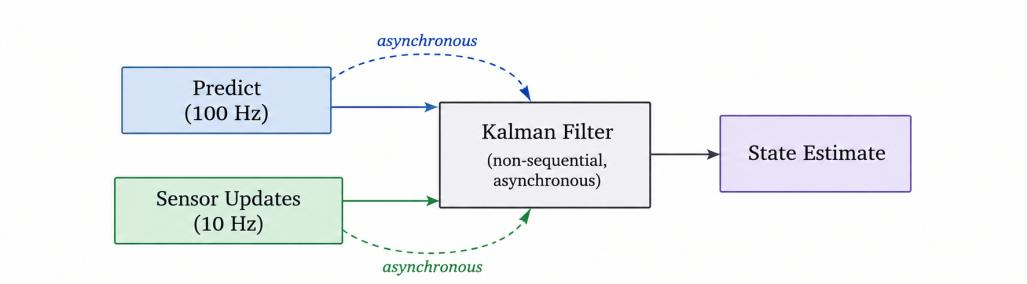
\includegraphics[width=\linewidth]{images/C5_8.png}
    \end{subfigure}\hfill
    \begin{subfigure}{0.5\textwidth}
        \centering
        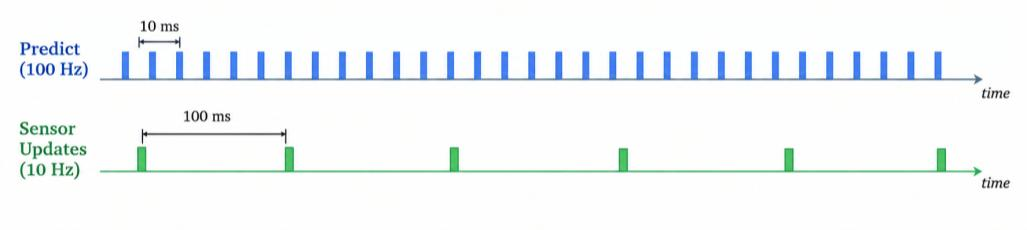
\includegraphics[width=\linewidth]{images/C5_9.png}
    \end{subfigure}
    \caption{Asynchronous: prediction at 100\,Hz, sensor updates at 10\,Hz}
\end{figure}

\begin{table}[H]
    \centering
    \begin{tabular}{|p{7.5cm}|p{7.5cm}|}
        \hline
        \textbf{Pros} & \textbf{Cons} \\
        \hline
        High-rate state output, set by the predict step & More complex to build: timestamps, buffers, threading \\
        \hline
        Every measurement is used as soon as it arrives & Delayed or out-of-order measurements need buffering and re-processing \\
        \hline
        Sensors are easy to add or remove (modular) & Accurate time synchronization across sensors is critical \\
        \hline
        Robust to a sensor dropping out & Uncertainty grows between corrections \\
        \hline
    \end{tabular}
    \caption{Asynchronous Kalman filter}
\end{table}

\subsection{The 1D Kalman filter}

\subsubsection{Gaussians}
\begin{wrapfigure}{R}{0.36\textwidth}
    \centering
    \vspace{-10pt}
    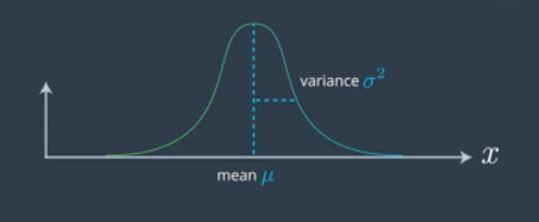
\includegraphics[width=0.35\textwidth]{images/C5_10.png}
    \caption{Mean and variance of a Gaussian}
    \vspace{-10pt}
\end{wrapfigure}
In a Kalman filter the state estimate is \textbf{always represented by a Gaussian} (normal) distribution, which models our \textbf{belief} about the true value of a variable, e.g.\ the position of a vehicle.
A Gaussian models continuous data where the values close to the mean are the most likely, and the area under the curve is 1 (the total probability):
\[
f(x) = \frac{1}{\sigma\sqrt{2\pi}} \exp\left(-\frac{(x-\mu)^2}{2\sigma^2}\right)
\]

A 1D Gaussian is described by only two parameters: the \textbf{mean} $\mu$ is the expected value, i.e.\ our \textbf{best estimate} of the state, while the \textbf{variance} $\sigma^2$ is the \textbf{uncertainty} around that estimate (how sure we are).
A larger $\sigma^2$ means a greater uncertainty, so obviously we want the variance to be as small as possible.
The Kalman filter continuously updates these two parameters, combining predictions and measurements, to keep the best possible estimate of the true state over time.

\begin{wrapfigure}{R}{0.36\textwidth}
    \centering
    \vspace{-10pt}
    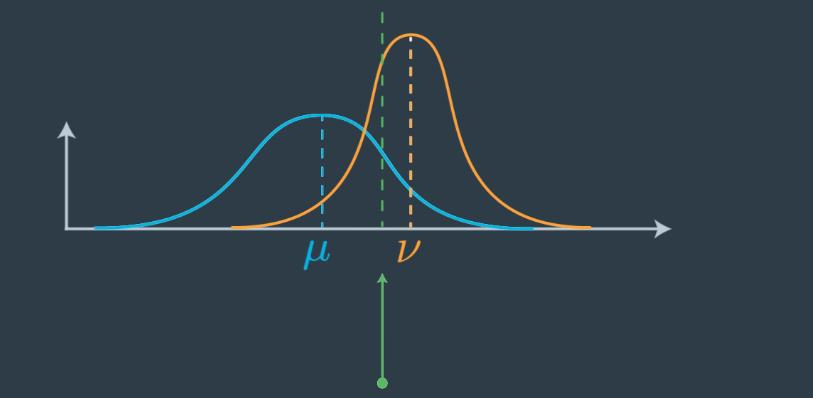
\includegraphics[width=0.35\textwidth]{images/C5_11.png}
    \caption{Prior ($\mu$) and new measurement ($\nu$)}
    \vspace{-10pt}
\end{wrapfigure}
For example, suppose we are computing the position of a vehicle: our current belief is a Gaussian whose mean is the estimated position $\mu$ and whose variance is our uncertainty.
A new measurement $\nu$ gives us information with a small variance, and combining it with the \textbf{prior} distribution we obtain an improved estimate, the \textbf{posterior}.
When we update the state we are therefore combining (multiplying) Gaussians, and the question is: how does the new Gaussian look like after fusing the two sources of information?

\subsubsection{Variables of the 1D filter}
\begin{table}[H]
    \centering
    \begin{tabular}{|c|p{12cm}|}
        \hline
        \textbf{Symbol} & \textbf{Meaning} \\
        \hline
        \multicolumn{2}{|l|}{\textit{State and motion (prediction)}} \\
        \hline
        $\mu_{prior}$ & Mean of the previous state, i.e.\ the current best estimate \\
        \hline
        $\sigma^2_{prior}$ & Variance of the previous state (uncertainty) \\
        \hline
        $u$ & Displacement/control applied by the kinematic model (e.g.\ $velocity \times \Delta t$) \\
        \hline
        $\sigma^2_u$ & Variance of the process/motion noise (uncertainty of the model) \\
        \hline
        \multicolumn{2}{|l|}{\textit{Sensor and update}} \\
        \hline
        $z$ & Value measured by the sensor (e.g.\ the position read by the GPS) \\
        \hline
        $\sigma^2_m$ & Variance of the measurement noise (uncertainty of the sensor) \\
        \hline
        $\mu_{new}$ & New estimated mean (posterior) \\
        \hline
        $\sigma^2_{new}$ & New updated variance \\
        \hline
        $K$ & Kalman gain: weight of the combination between model and sensor \\
        \hline
    \end{tabular}
    \caption{Variables of the 1D Kalman filter}
\end{table}

\subsubsection{Ground truth}
\noindent\begin{minipage}[c]{0.5\textwidth}
The \textbf{ground truth} $x$ is the \textbf{real trajectory} of the vehicle.
The filter does not know it: we only use it to \textbf{evaluate} the estimate $\hat{x}$, computing the error $e = x - \hat{x}$.

\vspace{4pt}On a real car the ground truth is not available: it is obtained from simulations, annotated datasets or reference sensors (e.g.\ RTK-GPS).
\end{minipage}\hfill
\begin{minipage}[c]{0.4\textwidth}
    \centering
    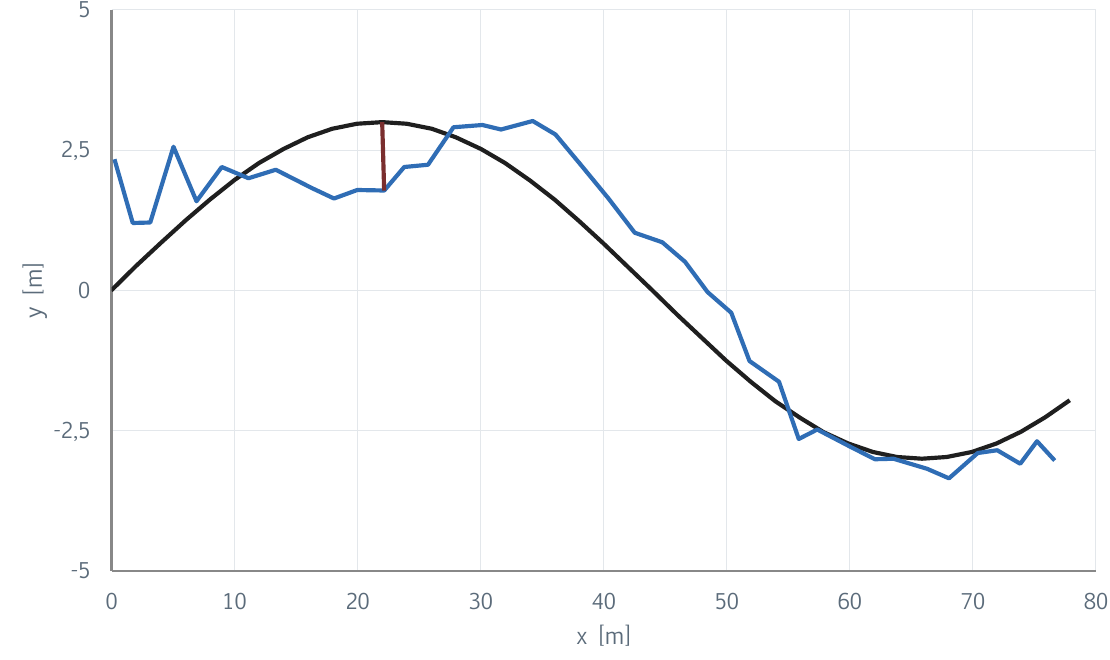
\includegraphics[width=\linewidth]{images/C5_12.png}
    \captionof{figure}{Ground truth (black), estimate (blue) and error (red)}
\end{minipage}

\subsubsection{Prediction}
The \textbf{prediction} step produces the estimate of the current variables \textbf{considering the uncertainties}.
The estimate is based on a \textbf{motion model}, which models how we believe the system evolves over time; here we use the information of the motion, for instance the velocity of the car.

We update the prior estimate by adding the effect of the motion, $new\_position = old\_position + u$, with $u = velocity \times time$.
Mathematically, this is equivalent to \textbf{adding two Gaussians}:
\[
\mu_{pred} = \mu_{prior} + u \qquad\qquad \sigma^2_{pred} = \sigma^2_{prior} + \sigma^2_u
\]
The new variance is the sum of the prior variance and of the variance of the motion model (how accurately we know the motion).
As a result, \textbf{the uncertainty always grows} during the prediction, because we lose precision when predicting: the Gaussian becomes wider and wider over time.
The figure below shows that the prediction is always wider than the previous state, and how much wider depends on how precise the motion model is (the process noise $Q$, i.e.\ $\sigma^2_u$).

\begin{figure}[H]
    \centering
    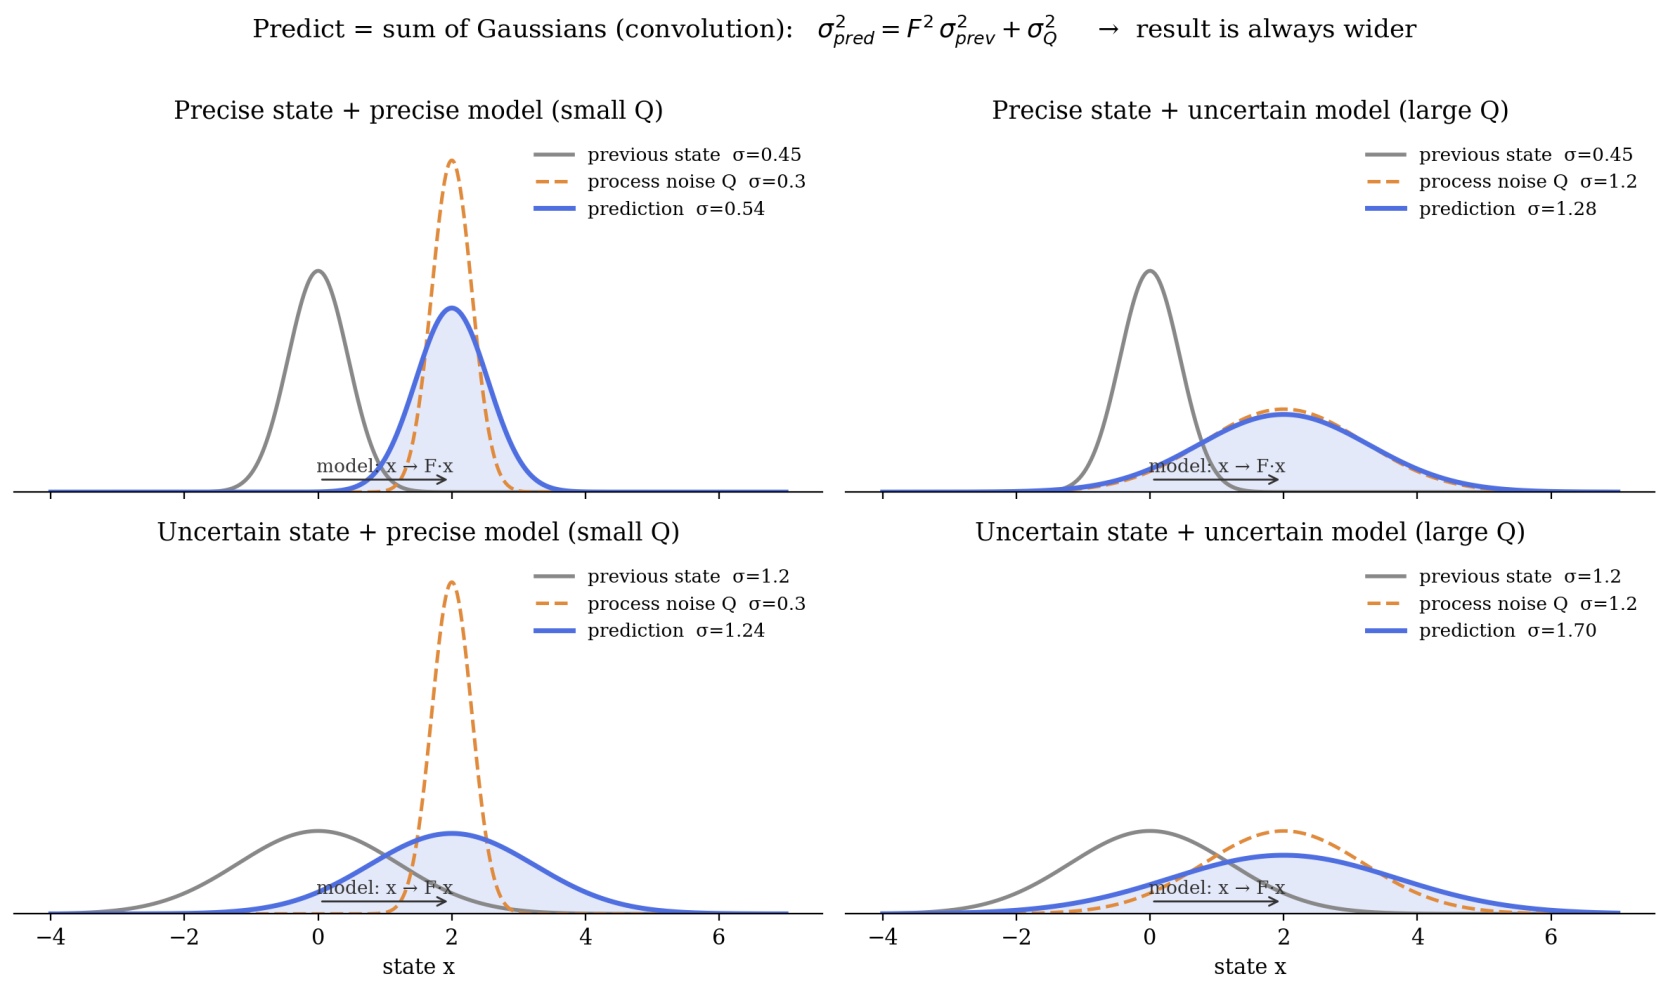
\includegraphics[width=0.7\textwidth]{images/C5_13.png}
    \caption{Prediction effects: precise/uncertain state with precise/uncertain model}
\end{figure}

\subsubsection{Kalman gain}
\noindent\begin{minipage}[c]{0.68\textwidth}
The \textbf{Kalman gain} $K$ decides \textbf{whom to trust}: the new sensor measurement or our motion model?
It is a scalar bounded between 0 and 1:
\[
K = \frac{\sigma^2_{pred}}{\sigma^2_{pred} + \sigma^2_m} \in [0, 1]
\]
\end{minipage}\hfill
\begin{minipage}[c]{0.28\textwidth}
    \centering
    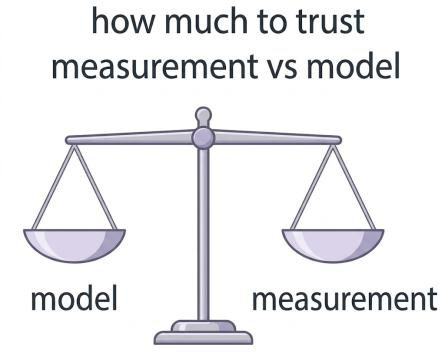
\includegraphics[width=\linewidth]{images/C5_14.png}
\end{minipage}

\vspace{6pt}A \textbf{high} Kalman gain ($K \to 1$) means that we \textbf{trust the measurement}: it happens when the sensor noise is very low, and the new estimate moves towards the measured value $z$.
A \textbf{low} Kalman gain ($K \to 0$) means that we \textbf{trust the prediction}: it happens when the sensor noise is very high, and the new estimate stays close to the predicted value $\mu_{pred}$.

\begin{infobox}[What if we have more sensors?]
In the slides we assume to have a single sensor, but in a real vehicle we usually have many (e.g.\ GPS and LiDAR). There are two standard ways to handle them:
\begin{compactitemize}
    \item \textbf{Sequential updates}: after the prediction, we apply one update for each sensor, each one with its own noise $\sigma^2_{m,i}$ (and therefore its own Kalman gain). The posterior of the first update becomes the prior of the second one, and so on. If the sensor noises are independent, the order does not matter and the result is the same as fusing all the measurements together. This is also what naturally happens in the \textbf{asynchronous} implementation: each sensor triggers an update when its measurement arrives.
    \item \textbf{Joint update}: all the measurements are stacked together and fused in a single update. In 1D the precisions simply add up: $\frac{1}{\sigma^2_{new}} = \frac{1}{\sigma^2_{pred}} + \sum_i \frac{1}{\sigma^2_{m,i}}$. In the multi-dimensional filter this is done by stacking the measurements in the vector $z$ and building the matrices $H$ and $R$ accordingly.
\end{compactitemize}
In both cases the more precise sensor automatically gets more weight, because of its higher Kalman gain.
\end{infobox}

\subsubsection{Correction (update)}
The goal of the correction is to use the information of the \textbf{sensors} (measurement model) to correct our prior estimate.
We combine the measurement with the prediction through the \textbf{product of two Gaussians}:
\[
\mu_{new} = \mu_{pred} + K \cdot \underbrace{(z - \mu_{pred})}_{innovation} \qquad\qquad \sigma^2_{new} = (1 - K) \cdot \sigma^2_{pred}
\]
The term $z - \mu_{pred}$ is called \textbf{innovation}: it is the difference between what the sensor measured and what the model predicted.
The new mean is therefore a weighted combination of the prediction and of the measurement: since the measurement usually has a lower uncertainty than the prediction, the new mean is closer to $z$.
Moreover, the new variance is \textbf{always smaller} than both the prediction and the measurement variances: with the update we \textbf{gain information and reduce the uncertainty}.

\begin{figure}[H]
    \centering
    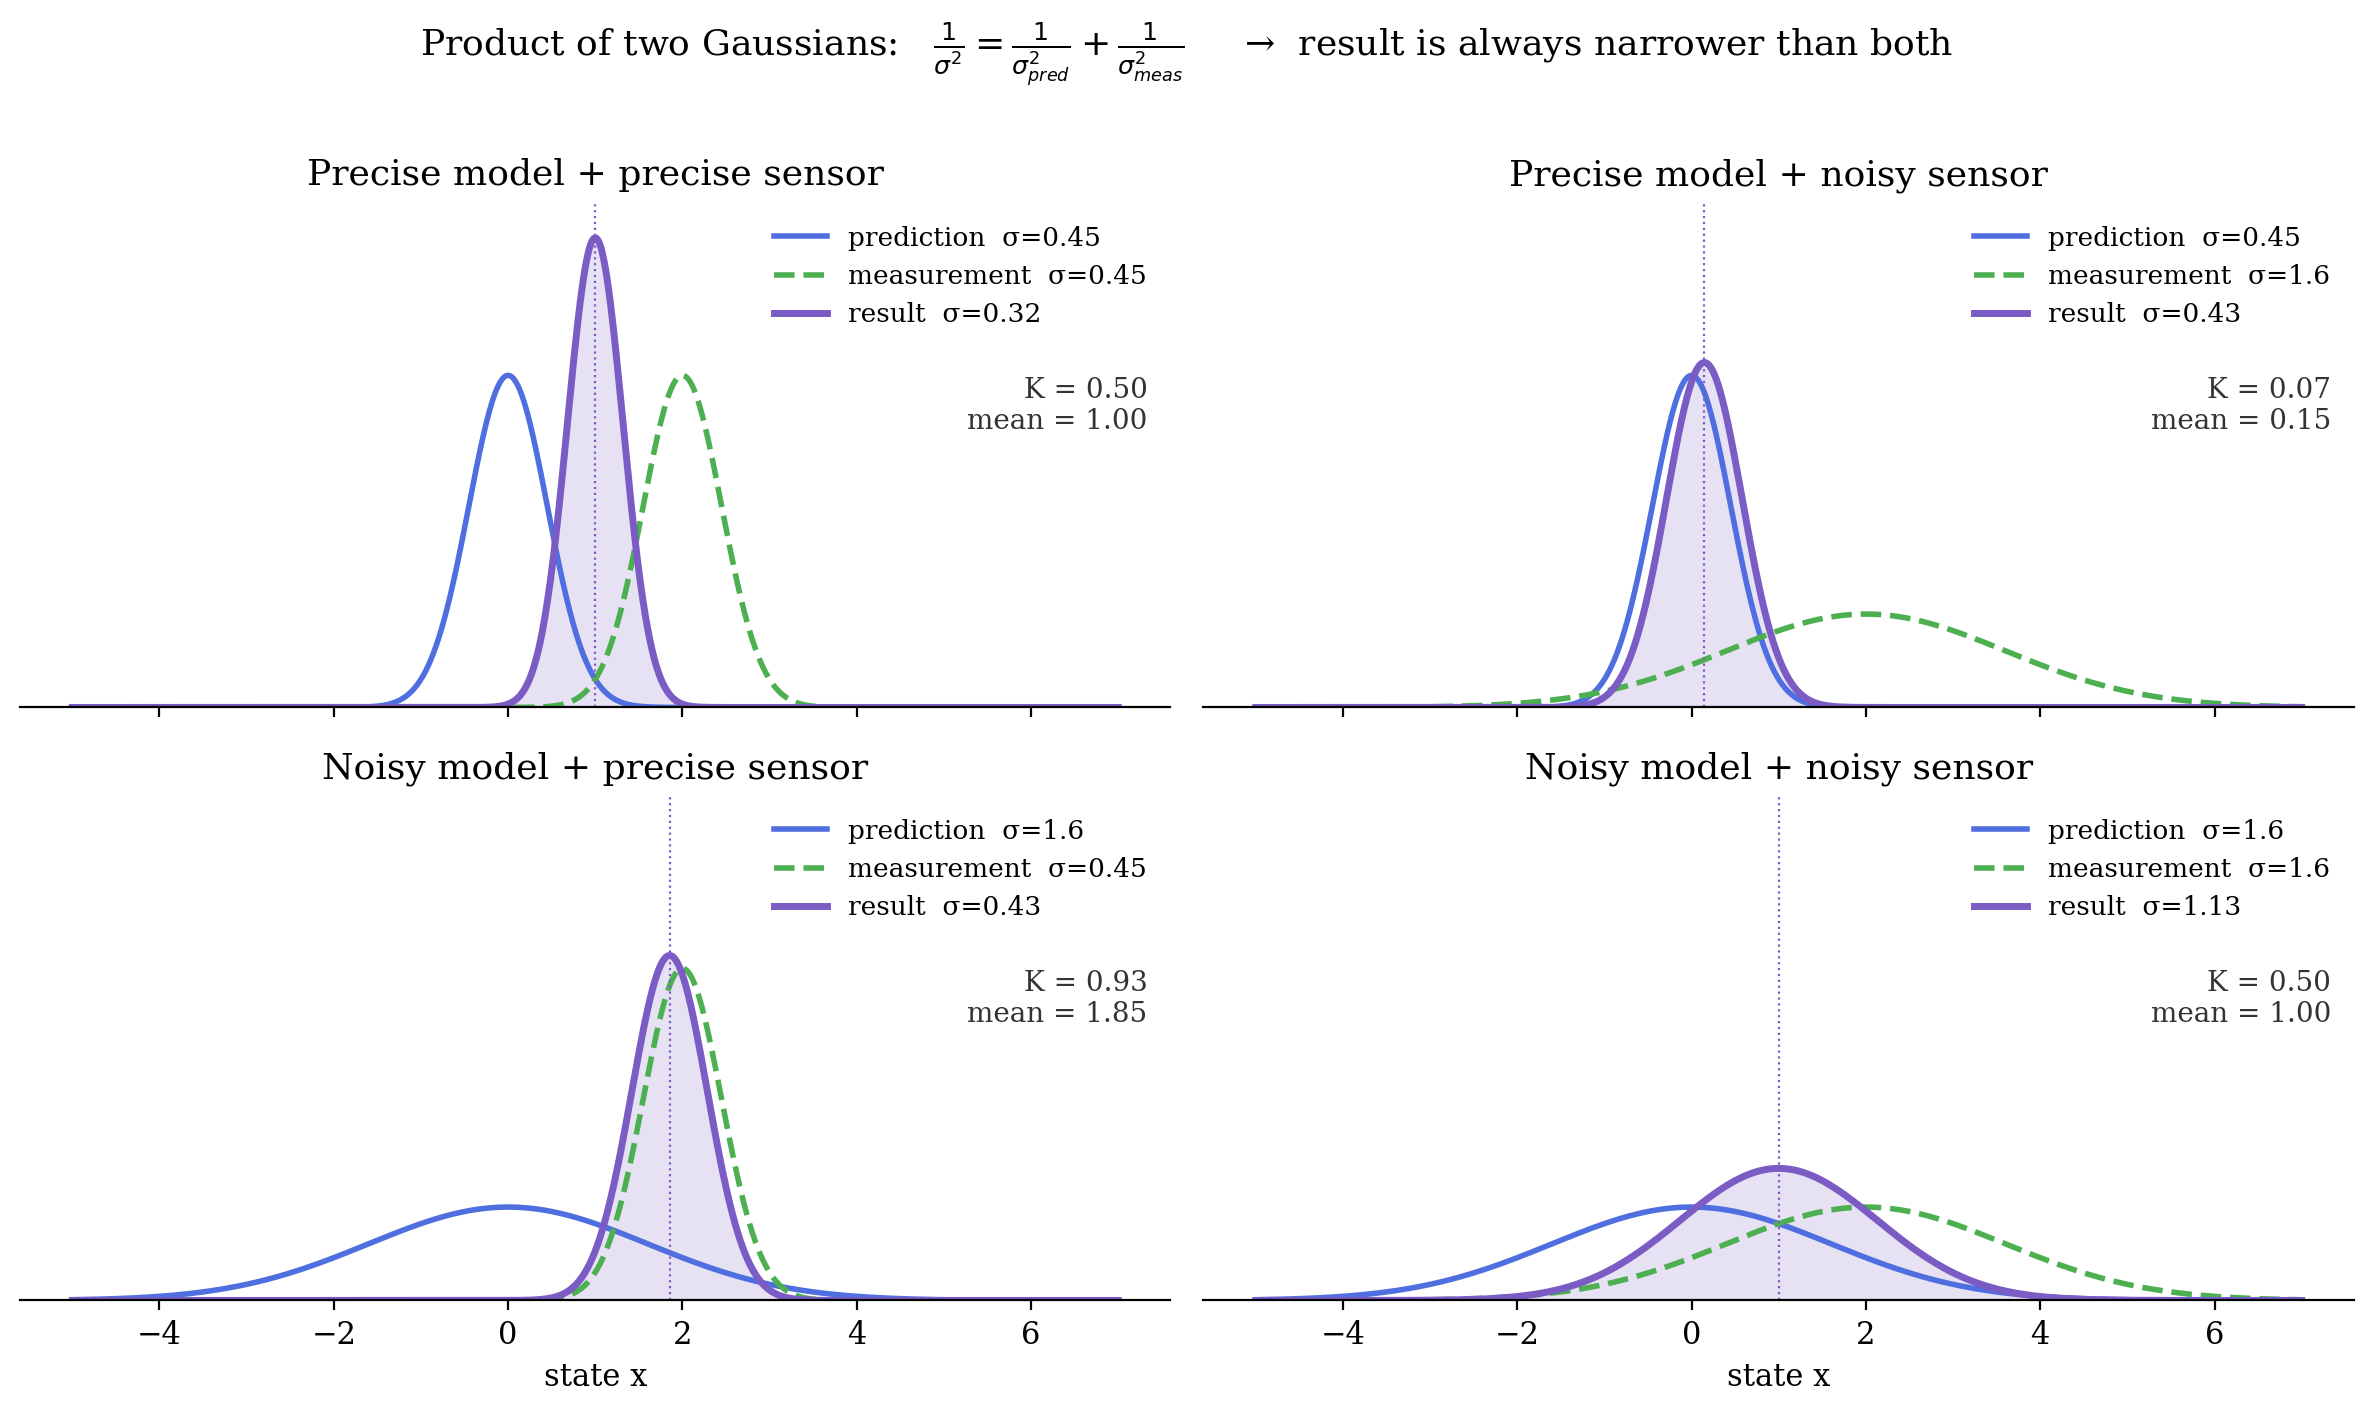
\includegraphics[width=0.7\textwidth]{images/C5_15.png}
    \caption{Update effects: the result is always narrower than both Gaussians}
\end{figure}

The same equations are often written directly as the product of the prior $(\mu, \sigma^2)$ and the measurement $(\nu, r^2)$:
\[
\mu' = \frac{r^2\mu + \sigma^2\nu}{r^2 + \sigma^2} \qquad\qquad \sigma^{2\,\prime} = \frac{1}{\frac{1}{r^2} + \frac{1}{\sigma^2}}
\]
which are exactly equivalent to the Kalman gain form above (with $\sigma^2 = \sigma^2_{pred}$, $\nu = z$ and $r^2 = \sigma^2_m$).

\begin{codicebox}[1D Kalman filter in Python]
\begin{lstlisting}
def predict(mu, sigma2, u, sigma2_u):
    # add the motion: the uncertainty grows
    return mu + u, sigma2 + sigma2_u

def update(mu, sigma2, z, sigma2_m):
    K = sigma2 / (sigma2 + sigma2_m)      # Kalman gain
    mu_new = mu + K * (z - mu)            # correct with the innovation
    sigma2_new = (1 - K) * sigma2         # the uncertainty shrinks
    return mu_new, sigma2_new

mu, sigma2 = 0.0, 1000.0                  # we know nothing at the start
for z, u in zip(measurements, motions):
    mu, sigma2 = predict(mu, sigma2, u, sigma2_u=2.0)
    mu, sigma2 = update(mu, sigma2, z, sigma2_m=4.0)
\end{lstlisting}
\end{codicebox}

\subsection{From 1D to multi-dimensional Kalman filter}
In the 1D filter the velocity was \textbf{given}, as a known input $u = v \cdot \Delta t$.
But what happens if the sensor measures \textbf{only the position}?
The Kalman filter allows us to estimate also quantities that are never measured directly, like the velocity: it is a \textbf{hidden variable}, contained in how the position changes over time.

\noindent\begin{minipage}[c]{0.5\textwidth}
\small
\begin{tabular}{|l|p{2cm}|p{2.6cm}|}
    \hline
     & \textbf{1D} & \textbf{Multi-dim.} \\
    \hline
    State & $\mu$ = position & $x = [p, v]^T$ \\
    \hline
    Velocity & known input $u = v\Delta t$ & estimated, never measured \\
    \hline
    Uncertainty & $\sigma^2$: one number & $P$: $2\times2$ matrix \\
    \hline
    Kalman gain & $K \in [0,1]$ & $K$: one gain per state variable \\
    \hline
\end{tabular}
\end{minipage}\hfill
\begin{minipage}[c]{0.46\textwidth}
    \centering
    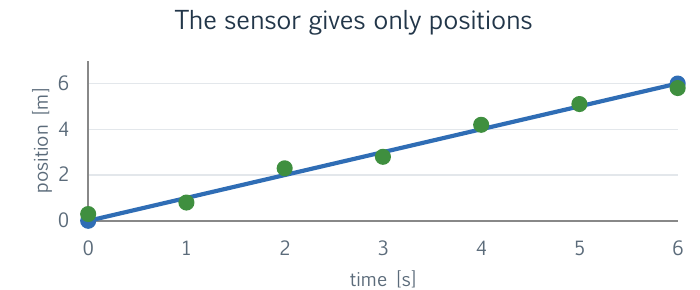
\includegraphics[width=\linewidth]{images/C5_16.png}
    \captionof{figure}{Measured positions (green): the velocity is their slope}
\end{minipage}

\vspace{6pt}To describe a state with more variables and their relationships we need \textbf{multivariate Gaussians}.

\subsubsection{Multivariate Gaussian}

The \textbf{multivariate Gaussian} is the generalization of the 1D normal distribution to more dimensions.
The mean $\mu$ becomes a \textbf{vector}, with one element for each dimension (e.g.\ $[position, velocity]$, both for the prediction and for the sensor model).
The variance becomes a $D\times D$ \textbf{covariance matrix}, which describes the relationships between the variables: on the diagonal we have the \textbf{variances} (the uncertainty of each variable), outside the diagonal the \textbf{covariances}, which measure how the estimation errors of two variables vary together.

\vspace{6pt}In the prediction model the covariance captures the uncertainty of the state and the relationships between variables like position and velocity, while in the sensor model it represents the noise of the sensors used to measure the state.

\paragraph{Covariance}
Covariance answers one question: if one variable is above its mean, where is the other one likely to be?
If the covariance is zero, knowing one variable tells nothing about the other; if it is positive, when one is high the other tends to be high too; if it is negative, when one is high the other tends to be low.

\begin{figure}[H]
    \centering
    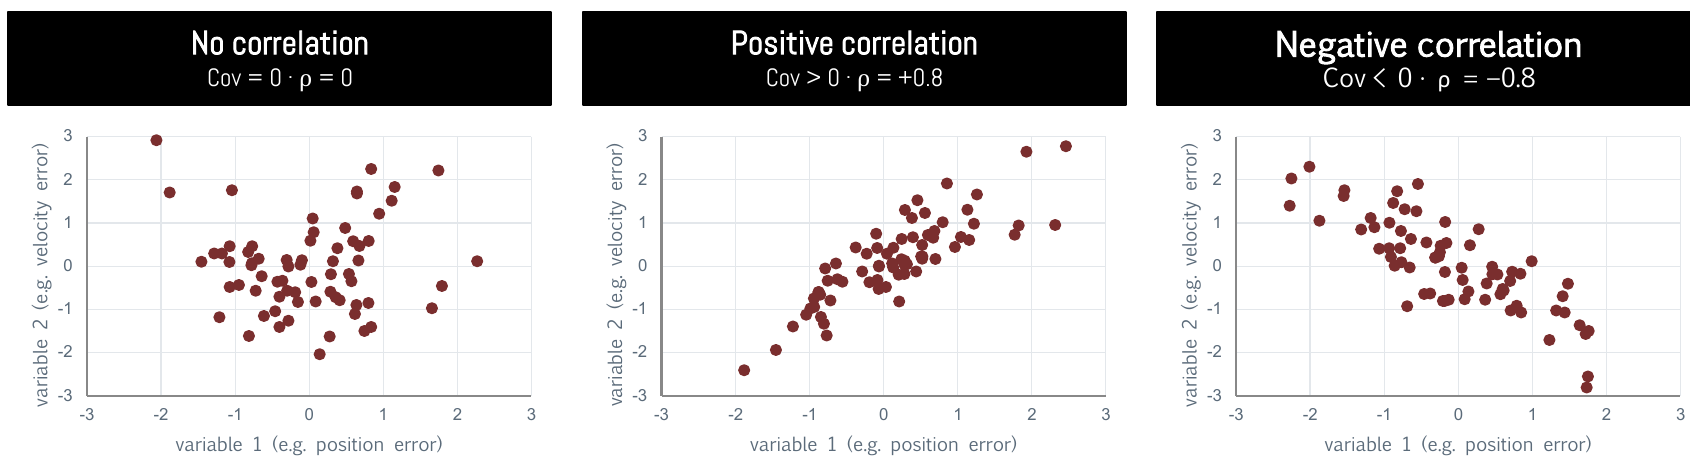
\includegraphics[width=0.85\textwidth]{images/C5_17.png}
    \caption{No correlation, positive correlation and negative correlation}
\end{figure}

In the Kalman filter the two variables are the \textbf{position error} and the \textbf{velocity error}, and their correlation is exactly what lets a \textbf{position measurement also correct the velocity}.

\paragraph{The covariance matrix $P$}
The Kalman filter does not know the state with certainty: it associates it with a variance-covariance matrix $P$, which represents the uncertainty (estimate error) of the system.
For a state $x = [p, v]^T$:
\[
P = \begin{bmatrix} V(p) & COV(p,v) \\ COV(v,p) & V(v) \end{bmatrix}
\]
\begin{compactitemize}
    \item $P[0,0]$ is the variance of the \textbf{position error} [m$^2$];
    \item $P[1,1]$ is the variance of the \textbf{velocity error} [(m/s)$^2$];
    \item $P[0,1] = P[1,0]$ tell us how the two errors are linked: if $P[0,1] > 0$ and we overestimate the velocity, we probably overestimate the position too; if $P[0,1] < 0$, when we overestimate one we probably underestimate the other; if $P[0,1] = 0$ the errors are unrelated.
\end{compactitemize}

\begin{examplebox}[Reading $P$]
Suppose the estimated state is $x = [50\,\text{m},\ 10\,\text{m/s}]^T$ with
$P = \begin{bmatrix} 0.04 & 0.05 \\ 0.05 & 0.25 \end{bmatrix}$.
The position has variance 0.04\,m$^2$, so $\sigma_p = \sqrt{0.04} = 0.20$\,m ($\approx\pm20$\,cm); the velocity has variance 0.25\,(m/s)$^2$, so $\sigma_v = 0.50$\,m/s.
The covariance 0.05\,m$^2$/s is positive: the errors are correlated, with correlation coefficient $\rho = 0.05 / (0.20 \cdot 0.50) = 0.5$.
So the Kalman filter does not only estimate \textbf{where} the car is, but also \textbf{how uncertain} the estimate is and \textbf{how the uncertainties are correlated}.
\end{examplebox}

\subsubsection{The Kalman filter equations}
The multi-dimensional filter is described by five equations, two for the prediction and three for the update.

\textbf{Prediction}:
\[
x' = Fx + u \qquad\qquad P' = FPF^T + Q
\]
The \textbf{state extrapolation} equation predicts the future state starting from the current estimate $x$; the \textbf{covariance extrapolation} equation gives the uncertainty of this prediction.

\textbf{Update}:
\[
y = z - Hx \qquad S = HPH^T + R \qquad K = PH^TS^{-1} \qquad x' = x + Ky \qquad P' = (I - KH)P
\]
First we compute the \textbf{innovation} $y$ and its covariance $S$, then the \textbf{Kalman gain} $K$, which weights the measurement against the past estimate; finally the \textbf{state update} gives the new estimate and the \textbf{covariance update} gives its uncertainty, used in the next prediction step.
As in 1D, if $K$ is close to 1 we give weight to the measurement, if it is close to 0 we give weight to the estimate.

\begin{table}[H]
    \centering
    \small
    \begin{tabular}{|c|l|c|p{6.8cm}|c|}
        \hline
        \textbf{Symbol} & \textbf{Name} & \textbf{Size} & \textbf{Meaning (example with $p$, $v$)} & \textbf{In 1D} \\
        \hline
        \multicolumn{5}{|l|}{\textit{Prediction}} \\
        \hline
        $x$ & State vector & $n\times1$ & $[position, velocity]^T$ & $\mu$ \\
        \hline
        $P$ & State covariance & $n\times n$ & uncertainty of $p$ and $v$ and covariance of their errors & $\sigma^2$ \\
        \hline
        $F$ & State transition matrix & $n\times n$ & $\begin{bmatrix}1 & \Delta t\\ 0 & 1\end{bmatrix}$: $p' = p + v\Delta t$, $v' = v$ & $\mu + u$ \\
        \hline
        $u$ & Control input & $n\times1$ & known external input (e.g.\ a braking command) & $u$ \\
        \hline
        $Q$ & Process noise covariance & $n\times n$ & how wrong the motion model can be & $\sigma^2_u$ \\
        \hline
        \multicolumn{5}{|l|}{\textit{Update}} \\
        \hline
        $z$ & Measurement & $m\times1$ & the position measured by the sensor & $z$ \\
        \hline
        $H$ & Measurement matrix & $m\times n$ & $[1, 0]$: the sensor sees $p$, not $v$ & -- \\
        \hline
        $R$ & Measurement noise cov. & $m\times m$ & sensor noise & $\sigma^2_m$ \\
        \hline
        $y$ & Innovation & $m\times1$ & $z - Hx$: the surprise & $z - \mu_{pred}$ \\
        \hline
        $S$ & Innovation covariance & $m\times m$ & $HPH^T + R$: how big the surprise is expected to be & $\sigma^2_{pred} + \sigma^2_m$ \\
        \hline
        $K$ & Kalman gain & $n\times m$ & $[K_p, K_v]^T$: turns the surprise into a correction of $p$ and $v$ & $K$ \\
        \hline
        $I$ & Identity matrix & $n\times n$ & used in $P' = (I - KH)P$ & 1 \\
        \hline
    \end{tabular}
    \caption{Variables of the multi-dimensional Kalman filter ($n$ = state variables, here 2; $m$ = measured quantities, here 1)}
\end{table}

\paragraph{Prediction design}
In the prediction, $x$ contains all the variables (states) of the system, e.g.\ position and velocity, and $x'$ is how the state propagates.
$P$ holds the current uncertainty of the states.
$F$ is the \textbf{state transition matrix}: it models how the system evolves over time.
With the \textbf{constant velocity model} (the object moves in a straight line at constant speed) we have $p' = p + v\Delta t$ and $v' = v$, that is:
\[
\begin{bmatrix} p' \\ v' \end{bmatrix} = \begin{bmatrix} 1 & \Delta t \\ 0 & 1 \end{bmatrix} \begin{bmatrix} p \\ v \end{bmatrix}
\]
$u$ is the \textbf{control vector}, which describes how the object changes because of internal or external forces (friction of the tires, gravity) or deterministic control inputs (e.g.\ the contribution of a spoiler).
$Q$ is the \textbf{process noise} covariance, which models the uncertainty due to the system dynamics, unmodelled effects or random disturbances.
In $P' = FPF^T + Q$, the diagonal is the uncertainty of the prediction and the off-diagonal terms are the correlation between the variables.

\paragraph{Update design}
In the update, $z$ is the value measured by the sensors (here the position).
$H$ is the \textbf{measurement function}: it projects the state into the measurement space of the sensor, i.e.\ it says what is measured and how it relates to the state vector. Here $H = [1, 0]$: the 1 indicates that the measured position is directly related to the position in the state, the 0 that the velocity is not measured.
$y = z - Hx$ is the \textbf{innovation} (the surprise), the difference between the measured value and the predicted measurement.
$R$ is the \textbf{measurement noise} covariance (sensors are not perfect!), whose magnitude depends on many parameters, such as the calibration.
$S$ is the \textbf{innovation covariance}: it combines the uncertainty of the estimate ($P$) and the measurement noise ($R$), and quantifies how much we trust the innovation.
$K$ is the \textbf{Kalman gain}: the more error in the prediction, the more weight is given to the sensor, and vice versa.
Finally, $x'$ is the new state and $P'$ the new covariance, which also describes the correlation between the variables (e.g.\ if our velocity is high, we probably moved a lot).

\subsubsection{How the Kalman filter finds the velocity}
Let's see how the filter estimates a variable that is never measured.
A car moves at 1\,m/s, the sensor measures only the position ($z = 1, 2, 3$\,m) with $R = 1$, and $\Delta t = 1$\,s.
At the start the filter knows nothing: $p = 0$, $v = 0$ and $P = \text{diag}(1000, 1000)$.
Since $H = [1, 0]$, the two gains are computed from the predicted $P$ as $K_p = P_{pp}/(P_{pp}+R)$ and $K_v = P_{vp}/(P_{pp}+R)$.

\begin{table}[H]
    \centering
    \small
    \begin{tabular}{|c|c|c|c|c|c|c|p{3.2cm}|}
        \hline
        \textbf{Step} & \textbf{Pred.\ $p$} & \textbf{$z$} & \textbf{$y$} & \textbf{Gains} & \textbf{New $p$} & \textbf{New $v$} & \textbf{Why} \\
        \hline
        1 & 0.0\,m & 1\,m & +1.0 & $K_p \approx 1.00$, $K_v \approx 0.50$ & 1.00\,m & 0.50\,m/s & $p$ and $v$ equally uncertain: blame split in half \\
        \hline
        2 & 1.5\,m & 2\,m & +0.5 & $K_p \approx 1.00$, $K_v \approx 0.995$ & 2.00\,m & 1.00\,m/s & $p$ now well known: the error must come from $v$ \\
        \hline
        3 & 3.0\,m & 3\,m & $\approx 0$ & $K_p \approx 0.83$, $K_v \approx 0.50$ & 3.00\,m & 1.00\,m/s & no surprise: $p$ and $v$ confirmed \\
        \hline
    \end{tabular}
    \caption{The filter finds the velocity in three steps}
\end{table}

\noindent\begin{minipage}[c]{0.55\textwidth}
The update is again the \textbf{product of two Gaussians}, now in the (position, velocity) plane: $posterior \propto prior \times likelihood$.
Looking at step 2:
\begin{enumerate}
    \item \textbf{Prediction}: $p \approx 1$\,m is well known, while $v$ is not; every pair with $p \approx 1 + v\Delta t$ is plausible, so the prior is a thin \textbf{tilted band}. The tilt is the covariance.
    \item \textbf{Measurement}: the sensor says $p \approx 2$\,m and nothing about $v$, so the likelihood is a vertical band.
    \item \textbf{Product}: only the points compatible with both survive, i.e.\ the crossing at $p \approx 2$\,m, $v \approx 1$\,m/s.
\end{enumerate}
\end{minipage}\hfill
\begin{minipage}[c]{0.41\textwidth}
    \centering
    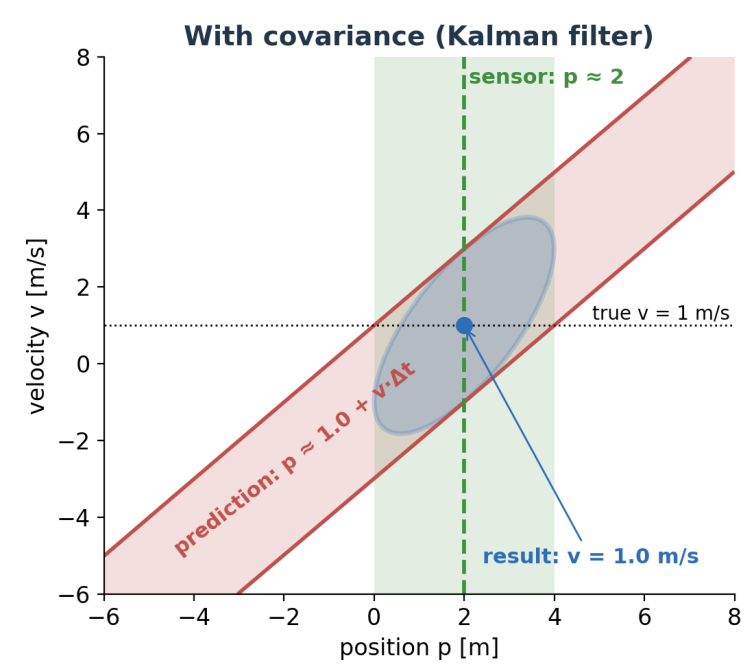
\includegraphics[width=\linewidth]{images/C5_19.png}
    \captionof{figure}{Update in the (position, velocity) plane}
\end{minipage}

\vspace{6pt}This is why the correlation between position and velocity errors is so important: without it, a position measurement could never correct the velocity.

\subsubsection{Motion models}
\textbf{Motion models} describe how the system evolves over time between two measurements: they predict the next state (position, velocity, \dots) from the previous one and from the known inputs (like control or acceleration), and they introduce a process uncertainty due to the model imperfections or to unknown influences.

\begin{table}[H]
    \centering
    \begin{tabular}{|l|c|l|p{5.3cm}|}
        \hline
        \textbf{Model} & \textbf{State} & \textbf{Transition equation} & \textbf{Assumption} \\
        \hline
        Constant position & $[p]$ & $p_k = p_{k-1}$ & The object is static; ideal for stationary targets \\
        \hline
        Constant velocity & $[p, v]$ & $\begin{aligned} p_k &= p_{k-1} + v_{k-1}\Delta t \\ v_k &= v_{k-1}\end{aligned}$ & Velocity is constant; ideal for regular, steady motion \\
        \hline
        Constant acceleration & $[p, v, a]$ & $\begin{aligned} p_k &= p_{k-1} + v_{k-1}\Delta t + \tfrac{1}{2}a_{k-1}\Delta t^2 \\ v_k &= v_{k-1} + a_{k-1}\Delta t\end{aligned}$ & Acceleration is constant; ideal for vehicles and dynamic agents \\
        \hline
    \end{tabular}
    \caption{Common motion models}
\end{table}
